\section{PLOT Plot Function}

\subsection{Usage}

This is the basic plot command for FreeMat.  The general syntax for its
use is
\begin{verbatim}
  plot(<data 1>,{linespec 1},<data 2>,{linespec 2}...,properties...)
\end{verbatim}
where the \verb|<data>| arguments can have various forms, and the
\verb|linespec| arguments are optional.  We start with the
\verb|<data>| term, which can take on one of multiple forms:
\begin{itemize}
\item  Vector Matrix Case -- In this case the argument data is a pair
    of variables.  A set of \verb|x| coordinates in a numeric vector, and a 
    set of \verb|y| coordinates in the columns of the second, numeric matrix.
    \verb|x| must have as many elements as \verb|y| has columns (unless \verb|y|
    is a vector, in which case only the number of elements must match).  Each
    column of \verb|y| is plotted sequentially against the common vector \verb|x|.

\item  Unpaired Matrix Case -- In this case the argument data is a 
    single numeric matrix \verb|y| that constitutes the \verb|y|-values
    of the plot.  An \verb|x| vector is synthesized as \verb|x = 1:length(y)|,
    and each column of \verb|y| is plotted sequentially against this common \verb|x|
    axis.

\item  Complex Matrix Case -- Here the argument data is a complex
    matrix, in which case, the real part of each column is plotted against
    the imaginary part of each column.  All columns receive the same line
    styles.

\end{itemize}
Multiple data arguments in a single plot command are treated as a \emph{sequence}, meaning
that all of the plots are overlapped on the same set of axes.
The \verb|linespec| is a string used to change the characteristics of the line.  In general,
the \verb|linespec| is composed of three optional parts, the \verb|colorspec|, the 
\verb|symbolspec| and the \verb|linestylespec| in any order.  Each of these specifications
is a single character that determines the corresponding characteristic.  First, the 
\verb|colorspec|:
\begin{itemize}
\item  \verb|'b'| - Color Blue

\item  \verb|'g'| - Color Green

\item  \verb|'r'| - Color Red

\item  \verb|'c'| - Color Cyan

\item  \verb|'m'| - Color Magenta

\item  \verb|'y'| - Color Yellow

\item  \verb|'k'| - Color Black

\end{itemize}
The \verb|symbolspec| specifies the (optional) symbol to be drawn at each data point:
\begin{itemize}
\item  \verb|'.'| - Dot symbol

\item  \verb|'o'| - Circle symbol

\item  \verb|'x'| - Times symbol

\item  \verb|'+'| - Plus symbol

\item  \verb|'*'| - Asterisk symbol

\item  \verb|'s'| - Square symbol

\item  \verb|'d'| - Diamond symbol

\item  \verb|'v'| - Downward-pointing triangle symbol

\item  \verb|'^'| - Upward-pointing triangle symbol

\item  \verb|'<'| - Left-pointing triangle symbol

\item  \verb|'>'| - Right-pointing triangle symbol

\end{itemize}
The \verb|linestylespec| specifies the (optional) line style to use for each data series:
\begin{itemize}
\item  \verb|'-'| - Solid line style

\item  \verb|':'| - Dotted line style

\item  \verb|'-.'| - Dot-Dash-Dot-Dash line style

\item  \verb|'--'| - Dashed line style

\end{itemize}
For sequences of plots, the \verb|linespec| is recycled with color order determined
by the properties of the current axes.  You can also use the \verb|properties|
argument to specify handle properties that will be inherited by all of the plots
generated during this event.  Finally, you can also specify the handle for the
axes that are the target of the \verb|plot| operation.
\begin{verbatim}
  handle = plot(handle,...)
\end{verbatim}
\subsection{Example}

The most common use of the \verb|plot| command probably involves the vector-matrix
paired case.  Here, we generate a simple cosine, and plot it using a red line, with
no symbols (i.e., a \verb|linespec| of \verb|'r-'|).
\begin{verbatim}
--> x = linspace(-pi,pi);
--> y = cos(x);
--> plot(x,y,'r-');
\end{verbatim}
which results in the following plot.


\centerline{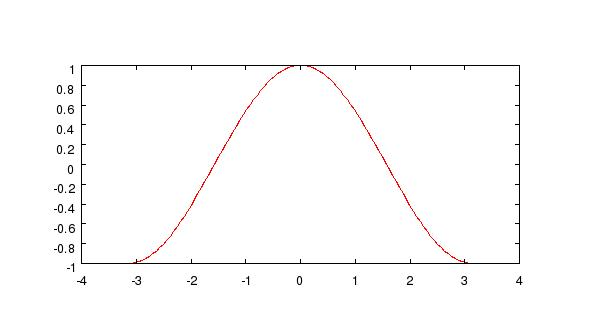
\includegraphics[width=8cm]{plot1}}


Next, we plot multiple sinusoids (at different frequencies).  First, we construct
a matrix, in which each column corresponds to a different sinusoid, and then plot
them all at once.
\begin{verbatim}
--> x = linspace(-pi,pi);
--> y = [cos(x(:)),cos(3*x(:)),cos(5*x(:))];
--> plot(x,y);
\end{verbatim}
In this case, we do not specify a \verb|linespec|, so that we cycle through the
colors automatically (in the order listed in the previous section).


\centerline{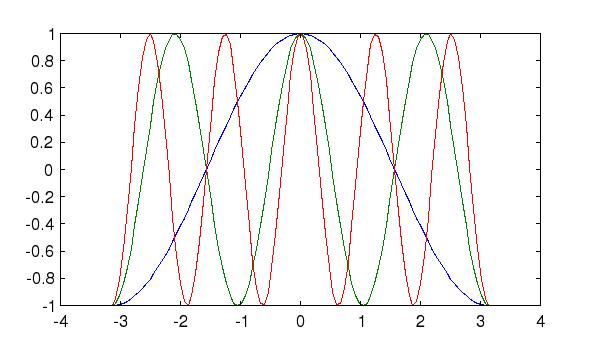
\includegraphics[width=8cm]{plot2}}


This time, we produce the same plot, but as we want to assign individual
\verb|linespec|s to each line, we use a sequence of arguments in a single plot
command, which has the effect of plotting all of the data sets on a common 
axis, but which allows us to control the \verb|linespec| of each plot. In 
the following example, the first line (harmonic) has red, solid lines with 
times symbols
marking the data points, the second line (third harmonic) has blue, solid lines
with right-pointing triangle symbols, and the third line (fifth harmonic) has
green, dotted lines with asterisk symbols.
\begin{verbatim}
--> plot(x,y(:,1),'rx-',x,y(:,2),'b>-',x,y(:,3),'g*:');
\end{verbatim}


\centerline{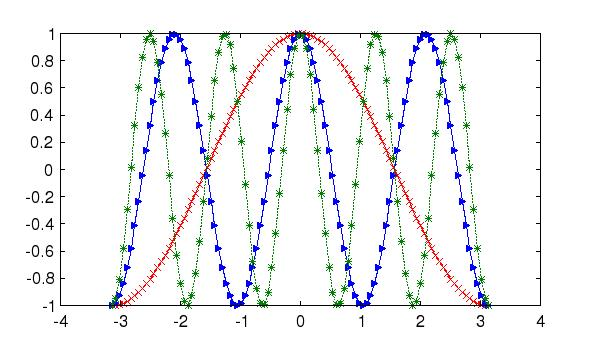
\includegraphics[width=8cm]{plot3}}


The second most frequently used case is the unpaired matrix case.  Here, we need
to provide only one data component, which will be automatically plotted against
a vector of natural number of the appropriate length.  Here, we use a plot sequence
to change the style of each line to be dotted, dot-dashed, and dashed.
\begin{verbatim}
--> plot(y(:,1),'r:',y(:,2),'b;',y(:,3),'g|');
\end{verbatim}
Note in the resulting plot that the \verb|x|-axis no longer runs from \verb|[-pi,pi]|, but 
instead runs from \verb|[1,100]|.


\centerline{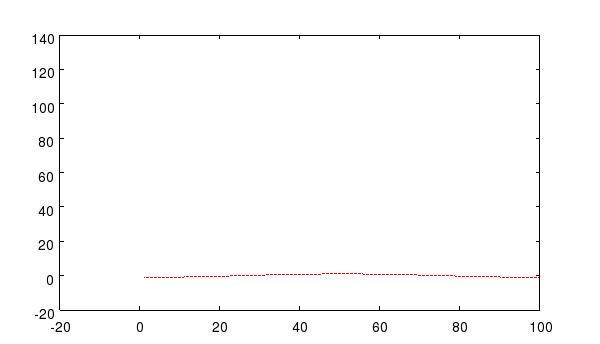
\includegraphics[width=8cm]{plot4}}


The final case is for complex matrices.  For complex arguments, the real part is
plotted against the imaginary part.  Hence, we can generate a 2-dimensional plot
from a vector as follows.
\begin{verbatim}
--> y = cos(2*x) + i * cos(3*x);
--> plot(y);
\end{verbatim}


\centerline{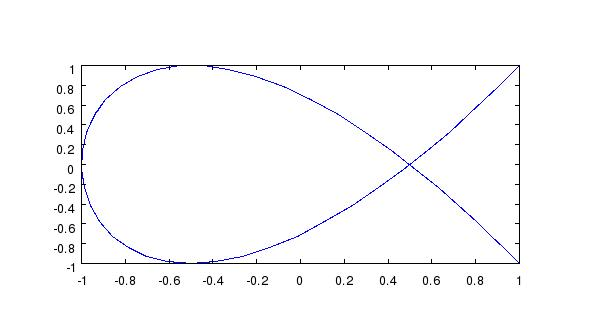
\includegraphics[width=8cm]{plot5}}


Here is an example of using the handle properties to influence the behavior
of the generated lines.
\begin{verbatim}
--> t = linspace(-3,3);
--> plot(cos(5*t).*exp(-t),'r-','linewidth',3);
\end{verbatim}


\centerline{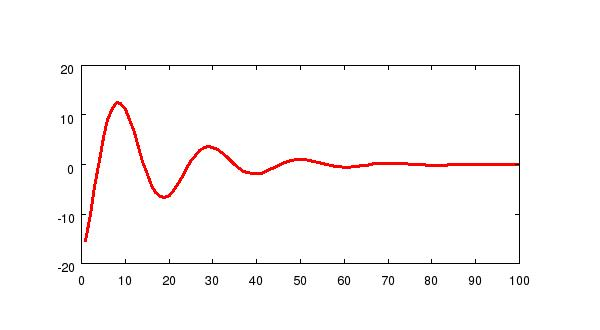
\includegraphics[width=8cm]{plot6}}

